\documentclass[conference]{IEEEtran}
\IEEEoverridecommandlockouts

\usepackage{cite}
\usepackage{amsmath,amssymb,amsfonts}
\usepackage{booktabs}
\usepackage{graphicx}
\usepackage{textcomp}
\usepackage{xcolor}
\usepackage{microtype}
\usepackage{url}
\usepackage{hyperref}
\usepackage[capitalise,noabbrev]{cleveref}

\hypersetup{colorlinks=false, pdfborder={0 0 0}, bookmarks=false}

% Ensure column gutter meets conference requirement (>= 0.2 in)
\setlength{\columnsep}{0.25in}
% Ensure top margin is at least 0.75 in on all pages
\setlength{\topmargin}{-0.25in}

\def\BibTeX{{\rm B\kern-.05em{\sc i\kern-.025em b}\kern-.08em
    T\kern-.1667em\lower.7ex\hbox{E}\kern-.125emX}}

\begin{document}

\title{BBR-SAT: Orbit-Aware Congestion Control\\
       for Multi-Orbit Satellite QUIC Handovers}

\author{
  \IEEEauthorblockN{Rajat Bhambani}
  \IEEEauthorblockA{
    \textit{Independent Research Contribution}\\
    bhambani.rajat@gmail.com
  }
}

\maketitle

% ── Abstract ──────────────────────────────────────────────────────────────────
\begin{abstract}
Low-Earth orbit (LEO), medium-Earth orbit (MEO), and geostationary (GEO)
satellite constellations are increasingly deployed together, creating
multi-orbit networks in which a single QUIC connection may traverse
orbit-class boundaries mid-flight.
Such handovers impose abrupt, step-change shifts in available bandwidth
(up to $5\times$ reduction) and round-trip time (up to $12\times$ increase),
which existing congestion-control algorithms handle poorly:
BBRv3 stalls for the duration of its two-cycle bandwidth filter, and
simple heuristics such as congestion-window freeze or send-pause succeed
only at a single, carefully tuned lead time.
We present \textbf{BBR-SAT}, a minimal extension of BBRv3 that equips the
sender with an orbit parameter table seeded from ephemeris data and a
two-phase handover protocol: a PREDICTED signal initiates a proactive queue
drain via ProbeBW\_DOWN, and a CONFIRMED signal resets the BDP context
directly from the orbit table.
Implemented in picoquic and evaluated in a zero-loss shared-link simulator
across all six pairwise LEO/MEO/GEO transitions at three handover times and
seven advance lead times, BBR-SAT converges to 90\% of new-orbit capacity
in 2.5\,s for the critical LEO$\to$GEO transition --- the only evaluated
mechanism to converge on this transition at any lead time from 0 to 20\,s ---
while reducing peak queue occupancy by $36\times$ relative to vanilla BBRv3.
Fairness analysis shows that BBR-SAT co-exists equitably with competing
BBRv3 flows (Jain $J = 0.997$) and neither worsens nor repairs the
pre-existing BBRv3 deference to CUBIC.
\end{abstract}

\begin{IEEEkeywords}
satellite communications, QUIC, congestion control, BBR, handover,
multi-orbit networks, LEO, GEO
\end{IEEEkeywords}

% ── I. Introduction ───────────────────────────────────────────────────────────
\section{Introduction}
\label{sec:intro}

The deployment of large LEO constellations (Starlink, OneWeb, Amazon
Kuiper)~\cite{handley2018delay,bhattacherjee2019}
alongside legacy MEO (O3b mPOWER) and GEO (ViaSat-3) infrastructure has
created a new class of network event: the \emph{inter-orbit handover}, in
which an active transport connection migrates between satellite beams
belonging to orbit classes with fundamentally different propagation
characteristics.
Such transitions are \emph{abrupt} --- the link properties change at the
granularity of a single RTT --- and \emph{asymmetric}:
a LEO$\to$GEO handover simultaneously reduces the available link rate by
$5\times$ (50$\to$10\,Mbps) and increases the round-trip propagation delay
by $\sim$$12\times$ (50$\to$580\,ms).
Because the GEO BDP (10\,Mbps$\times$580\,ms\,=\,725\,KB) exceeds the
LEO BDP (50\,Mbps$\times$50\,ms\,=\,312\,KB), the \emph{new} orbit requires
a \emph{larger} inflight window --- but at a \emph{much lower} pacing rate.

Modern QUIC stacks running BBRv3~\cite{cardwell2026bbr} are particularly
poorly suited to absorb this transition.
BBRv3's two-cycle \texttt{MaxBwFilter} requires approximately
$8 \times \mathrm{RTT}_\mathrm{new}$ to clear its pre-handover bandwidth
estimate.
On a GEO link ($\mathrm{RTT} \approx 580$\,ms) that amounts to roughly
5\,seconds of sustained over-pacing at 50\,Mbps into a 10\,Mbps pipe,
accumulating $\approx$33\,MB of queued data in our experiments before the
filter clears and the sender backs off.

The central insight motivating BBR-SAT is that satellite operators have
\emph{advance knowledge} of handover events: orbital mechanics are
deterministic, and ground-control systems routinely predict beam transitions
minutes ahead of time.
This knowledge can be surfaced to the transport layer as two signals:
(1)~PREDICTED, issued seconds to tens of seconds before the event, and
(2)~CONFIRMED, issued at the moment the beam switch completes.
BBR-SAT consumes these signals to execute a two-phase response:
a proactive queue drain aligned with the current (pre-handover) RTT,
followed by an instantaneous BDP context switch that seeds the post-handover
pacing rate and congestion window directly from a per-orbit parameter table.

This paper contributes: (1) the BBR-SAT algorithm --- two new signals,
an orbit parameter table, and a two-phase handover protocol integrated
into BBRv3 in $<$100 lines (\S\ref{sec:design}); (2) a zero-loss
shared-link simulator spanning all six pairwise orbit transitions at
three handover times and six lead times (\S\ref{sec:methodology});
and (3) empirical demonstration that BBR-SAT is the only evaluated
mechanism to converge at the critical LEO$\to$GEO transition across
lead times 0--20\,s, with fairness results confirming that advance
knowledge does not translate into a bandwidth advantage
(\S\S\ref{sec:exp1}--\ref{sec:fairness}).

% ── II. Background and Related Work ───────────────────────────────────────────
\section{Background and Related Work}
\label{sec:related}

\subsection{BBRv3 Filter Mechanics}

BBR~\cite{cardwell2016bbr} drives the sender at the estimated bottleneck
bandwidth using two long-term filters.
The \texttt{MaxBwFilter} is a two-slot windowed maximum over the last two
ProbeBW cycles; each cycle spans $\sim$4\,RTTs, so on a GEO link
(RTT\,$\approx$\,580\,ms) clearing a stale pre-handover estimate takes
$8 \times 580 \approx 4{,}640$\,ms.
The \texttt{min\_rtt} filter holds the minimum observed RTT over a
10-second window; a LEO$\to$GEO transition (50$\to$580\,ms) leaves the
sender calibrated to the wrong path delay for up to 10\,s.
BBRv3~\cite{cardwell2026bbr} adds \texttt{bw\_hi} (long-term
delivery-rate ceiling) and \texttt{inflight\_hi} (loss-driven inflight
limit), neither of which adapts on the timescale of a beam switch.

\subsection{Prior Work on Satellite Handover CCA}

Five intra-LEO cross-layer mechanisms appeared in 2024--2025:
StarQUIC~\cite{zhao2024starquic}, SATPIPE~\cite{zhao2025satpipe},
LeoCC~\cite{lai2025leocc}, Creo~\cite{yan2025creo},
and OrbCC~\cite{valentine2025orbcc}; Table~\ref{tab:related} summarises
their signal and algorithmic approach.
All operate within a single LEO constellation and none handle cross-orbit
transitions between orbit classes with fundamentally different propagation
regimes.

At the IETF, Lai et al.~\cite{lai2026lsncc} (draft-lai-ccwg-lsncc-01)
define the \emph{Path Phase Boundary} (PPB): an advisory signal that
path conditions may have changed discontinuously.
PPB is reactive, parameter-free, and CCA-agnostic --- it identifies the
problem but prescribes no algorithmic response.
Careful Resume~\cite{kuhn2025carefulresume} (draft-ietf-tsvwg-careful-resume-24)
caches one (cwnd, RTT) observation per remote endpoint for fast connection
startup, but does not re-engage mid-connection.
Its only satellite evaluation tests CUBIC, not BBR~\cite{hofstatter2025crsat}.

BBR-SAT is motivated by the PPB problem statement but differs structurally:
it fires \emph{before} the event (predictive), carries the target orbit
class (parameterized), and triggers a specific BBRv3 state-machine response
(BDP context switch).
The defining gap it fills --- cross-orbit mid-connection BDP switching ---
is absent from all prior work.

\begin{table}[t]
\centering
\caption{Satellite handover CCA mechanisms}
\label{tab:related}
\footnotesize
\setlength{\tabcolsep}{3pt}
\begin{tabular}{lccl}
\toprule
Mechanism & Mid-Conn? & Cross-Orbit? & Signal \\
\midrule
PPB~\cite{lai2026lsncc}                       & reactive & No  & ICMP probe \\
Careful Resume~\cite{kuhn2025carefulresume}   & No       & No  & cached obs.\ \\
StarQUIC~\cite{zhao2024starquic}              & Yes      & No  & 15-s sched.\ \\
SATPIPE~\cite{zhao2025satpipe}                & Yes      & No  & NTP sched.\ \\
LeoCC~\cite{lai2025leocc}                     & Yes      & No  & ICMP probe \\
Creo~\cite{yan2025creo}                       & Yes      & No  & cross-layer \\
OrbCC~\cite{valentine2025orbcc}               & Yes      & No  & INT \\
\textbf{BBR-SAT}                              & Yes      & \textbf{Yes} & eph./INT/probe \\
\bottomrule
\end{tabular}
\end{table}

Legacy work addressed GEO-specific impairments: PEPs and
Hybla~\cite{caini2004hybla} improve TCP on high-latency links;
characterisation of LEO paths~\cite{bhattacherjee2019,michel2022starlink}
documents the dynamics that make inter-orbit transitions damaging.
RFC 9743/BCP~133~\cite{duke2025rfc9743} mandates fairness evaluation for
any new CCA; \S\ref{sec:fairness} satisfies this.

% ── III. System Design ────────────────────────────────────────────────────────
\section{BBR-SAT Design}
\label{sec:design}

\subsection{Orbit Parameter Table}

BBR-SAT augments the per-connection BBRv3 state with a three-entry
\emph{orbit table}, one entry per orbit class (LEO, MEO, GEO):

\begin{center}
\small
\setlength{\tabcolsep}{4pt}
\begin{tabular}{ll}
\toprule
Field & Meaning \\
\midrule
\texttt{min\_rtt\_us}   & Ephemeris-derived propagation RTT ($\mu$s) \\
\texttt{bw\_hi}         & Nominal beam capacity (bits/s) \\
\texttt{bw\_confidence} & \textsc{ephemeris} or \textsc{measured} \\
\bottomrule
\end{tabular}
\end{center}

Entries are populated at connection setup from satellite ephemeris data
supplied by the operator; the \texttt{bw\_confidence} field transitions
from \textsc{ephemeris} to \textsc{measured} once the algorithm has
accumulated one ProbeBW cycle on that orbit.
The \texttt{min\_rtt} field is trusted immediately because propagation delay
is deterministic given orbital geometry; the \texttt{bw\_hi} field is
treated as a starting ceiling, not a hard limit, allowing BBR's natural
probing to refine it.

\subsection{Signal Protocol}

Two signals are delivered to the congestion controller via the picoquic
\texttt{alg\_notify} callback, distinguished by the value carried in the
\texttt{nb\_bytes\_acknowledged} field:

\begin{itemize}
  \item \textbf{PREDICTED} (\texttt{0x32}): the ground control system
        predicts a handover to a target orbit within the next $\ell$ seconds.
        The signal identifies the target orbit index.
  \item \textbf{CONFIRMED} (\texttt{0x02}): the beam switch has completed;
        the sender is now on the target orbit.
\end{itemize}

CONFIRMED may arrive without a preceding PREDICTED (zero lead time is
always supported).

\subsection{Two-Phase Handover Protocol}

\textbf{Phase 1 --- Proactive Drain (PREDICTED signal).}
When BBR-SAT receives PREDICTED, it forces BBRv3 into
\texttt{ProbeBW\_DOWN} with the drain gain ($\eta < 1$) applied to the
current orbit's BDP.
The \texttt{bw\_probe\_ceiling} is set to $2 \times \texttt{max\_bw}$ to
suppress spurious re-Startup triggers during the drain.
Any recovery state (\texttt{is\_in\_recovery}, \texttt{is\_pto\_recovery},
\texttt{packet\_conservation}) is cleared to allow the drain to proceed
without interference from the loss-recovery path.
The drain completes within one to two RTTs of the \emph{current} orbit,
well before the handover fires for lead times up to $\approx$20\,s.

\textbf{Phase 2 --- BDP Context Switch (CONFIRMED signal).}
On CONFIRMED, BBR-SAT:
\begin{enumerate}
  \item Loads the target orbit's \texttt{min\_rtt\_us} and \texttt{bw\_hi}
        directly into the BBRv3 state, bypassing the
        \texttt{MaxBwFilter} and \texttt{min\_rtt} expiry windows.
  \item Resets \texttt{inflight\_hi} to
        $\texttt{bw\_hi} \times \texttt{min\_rtt\_us}$
        (one BDP of the new orbit).
  \item Clears both slots of the two-cycle \texttt{MaxBwFilter},
        forcing BBR to accept the seeded \texttt{bw\_hi} as the new
        bandwidth ceiling in the very next round.
  \item Enters \texttt{ProbeBW\_REFILL} to ramp up to the new BDP.
\end{enumerate}

The net effect is that the post-handover pacing rate reflects the new
orbit's capacity within one RTT of the CONFIRMED signal, rather than
the $8 \times \mathrm{RTT}_\mathrm{new}$ required for natural BBRv3
filter convergence.

% ── IV. Methodology ───────────────────────────────────────────────────────────
\section{Methodology}
\label{sec:methodology}

\subsection{Simulator}

All experiments use \texttt{picoquic\_ns}~\cite{huitema2023picoquic},
the built-in network simulator embedded in picoquic.
The simulator runs QUIC connections in discrete-event simulation time,
sharing a single bottleneck link defined by a \texttt{picoquic\_ns\_spec\_t}
structure.
We extended this structure with a \texttt{main\_signal\_time} and
\texttt{main\_signal\_value} field to fire PREDICTED and CONFIRMED signals
at deterministic simulation times.
A \texttt{vary\_link\_spec} array changes link parameters (rate, latency,
buffer) at \texttt{handover\_time\_s}, modelling the beam switch.

Single-flow experiments use one QUIC connection (server$\to$client bulk
transfer); fairness experiments use two connections sharing the same
bottleneck.
All simulations are zero-loss (no packet loss injection) to isolate the
congestion-control response from loss-recovery interactions.

\subsection{Orbit Parameters}
\label{sec:orbits}

\begin{table}[t]
\centering
\caption{Simulated orbit parameters}
\label{tab:orbits}
\small
\begin{tabular}{lrrr}
\toprule
Orbit & Link rate & RTT  & BDP \\
\midrule
LEO   & 50\,Mbps  & 50\,ms  & 312\,KB \\
MEO   & 30\,Mbps  & 150\,ms & 562\,KB \\
GEO   & 10\,Mbps  & 580\,ms & 725\,KB \\
\bottomrule
\end{tabular}
\end{table}

Table~\ref{tab:orbits} lists the parameters used for each orbit class.
We model the bottleneck with an uncapped queue (no drop-tail depth limit),
consistent with satellite ground-segment equipment that provisions large
buffers to avoid loss on high-BDP links~\cite{border2001rfc3135}.
A sender that fails to drain inflight data before the BDP step-change
builds an arbitrarily large queue; the 33\,MB peak for B1 is this failure.

\subsection{Baselines}

\begin{itemize}
  \item \textbf{B1} --- Vanilla BBRv3 (no modification, no signal).
  \item \textbf{B3} --- cwnd-freeze: congestion window is held constant
        from the PREDICTED signal until five RTTs after CONFIRMED.
        (B2, a delayed-reduction variant, produced results
        indistinguishable from B1 at all tested lead times and is omitted.)
  \item \textbf{B4} --- send-pause/resume: the sender pauses all
        transmissions on PREDICTED and resumes on CONFIRMED.
  \item \textbf{BBR-SAT} --- the proposed algorithm (this work).
  \item \textbf{CUBIC} --- standard CUBIC, no modification.
\end{itemize}

B3 and B4 are common heuristics proposed informally in the satellite
operator community; CUBIC serves as a loss-driven convergence reference.
In our prototype, PREDICTED and CONFIRMED signals are injected at the
application layer via picoquic's \texttt{alg\_notify} callback;
a production deployment would carry them in a QUIC DATAGRAM
frame~\cite{pauly2022rfc9221} or operator-defined transport parameter.

\subsection{Experiment Parameters}

\textbf{Experiment 1 (single-flow):}
Each baseline is run through all six pairwise orbit transitions
(LEO$\leftrightarrow$MEO, LEO$\leftrightarrow$GEO, MEO$\leftrightarrow$GEO)
at three handover times ($T_\mathrm{HO} \in \{30, 60, 120\}$\,s)
and six lead times ($\ell \in \{0, 2, 5, 10, 20, 30\}$\,s).
Total simulation: 90\,s per trial.

\textbf{Experiment 2 (fairness):}
Two-flow shared-bottleneck runs under two topologies:
\textbf{F1} --- both flows cross a LEO$\to$GEO handover at $T=30$\,s
(flow~1: BBR-SAT, flow~2: BBRv3 or CUBIC);
\textbf{F3} --- both flows start on GEO, BBR-SAT re-anchors its BDP
context at $T=30$\,s (flow~2: CUBIC).
Each condition is repeated twice; post-event averages are 2-run means.

% ── V. Evaluation ─────────────────────────────────────────────────────────────
\section{Evaluation}
\label{sec:evaluation}

% ── V-A: Single-Flow ──────────────────────────────────────────────────────────
\subsection{Single-Flow Handover Performance}
\label{sec:exp1}

\subsubsection{Setup}

We drive each of the five baselines through all six pairwise orbit
transitions (LEO$\leftrightarrow$MEO, LEO$\leftrightarrow$GEO,
MEO$\leftrightarrow$GEO) at three handover times
($T_\mathrm{HO} \in \{30, 60, 120\}$\,s) and six lead times
($\ell \in \{0, 2, 5, 10, 20, 30\}$\,s).
Each condition is a zero-loss, single-flow simulation; parameters for each
orbit are given in Table~\ref{tab:orbits}.
The primary metric is \textbf{T90}: the elapsed time from
$T_\mathrm{HO}$ until the delivered throughput first reaches
90\,\% of the new orbit's link capacity, measured as a one-second rolling
average.
A trial is declared \emph{not converged} (N/C) if T90 exceeds the
60-second post-handover window.
We additionally record post-handover steady-state throughput
(mean over $t \in (T_\mathrm{HO}+20, T_\mathrm{HO}+60]$\,s),
goodput (total bytes delivered in the 90-second run),
and peak on-path queue depth.

\subsubsection{LEO$\to$GEO: the Critical Transition}

A downward BDP transition --- lower link rate, higher latency, larger BDP
--- is the most demanding case.
Table~\ref{tab:exp1_leo_geo} and Figure~\ref{fig:t90_lead} show results
for the LEO$\to$GEO transition at $T_\mathrm{HO} = 30$\,s with $\ell = 0$.

\textbf{B1 (vanilla BBRv3)} fails entirely: the on-path queue inflates to
33\,MB (the full GEO buffer), steady-state throughput is effectively zero,
and the 90\% threshold is never reached within the 60-second window.
The root cause is that BBRv3 retains its LEO-calibrated bandwidth estimate
after handover.
Because BBRv3's two-cycle \texttt{MaxBwFilter} clears only after roughly
$8 \times \mathrm{RTT}_\mathrm{GEO} \approx 5$\,s~\cite{cardwell2026bbr},
the sender continues pacing at $\approx$50\,Mbps into a 10\,Mbps pipe,
sustaining a queue that grows without bound at the simulation's buffer limit.

\textbf{B3 (cwnd-freeze)} exhibits the same failure mode.
Freezing the congestion window at the pre-handover LEO value leaves an
equally oversized window in place; the buffer fills to 33\,MB
identically to B1.
Advance warning is useless: even at $\ell = 30$\,s, B3 does not converge.

\textbf{B4 (send-pause/resume)} converges exactly once across the full
lead-time sweep, at $\ell = 5$\,s (T90 = 5.6\,s), and fails at every
other lead time.
The narrow success window reflects the tight timing between the pause
duration and the GEO queue-drain time: too short a pause leaves residual
in-flight data that re-inflates the queue; too long a pause wastes capacity
and triggers a slow-start on resume.

\textbf{BBR-SAT} converges at every tested lead time from $\ell = 0$ to
$\ell = 20$\,s, with T90 = 2.5\,s throughout.
On receiving the CONFIRMED signal at $T_\mathrm{HO}$, the algorithm
loads the seeded GEO orbit entry (\texttt{bw\_hi} = 10\,Mbps, \texttt{min\_rtt}
= 580\,ms), enters a brief DRAIN phase to clear residual in-flight data,
then transitions to REFILL and converges to a steady-state of 9.2\,Mbps
(92\,\% of link capacity) with a peak queue of only 910\,KB --- a
$36\times$ reduction compared to B1/B3.
Goodput over the 90-second run is 56.9\,MB, largely independent of lead time.

At $\ell = 30$\,s, T90 degrades sharply to 47.6\,s.
The PREDICTED signal at $t = 0$\,s (i.e.\ $T_\mathrm{HO} - 30$\,s)
initiates a proactive queue drain via ProbeBW\_DOWN; however, because
the actual handover does not occur for 30\,s, BBR-SAT re-enters
ProbeBW\_UP and rebuilds a LEO-calibrated queue before the CONFIRMED
signal fires.
This establishes a practical upper bound: lead times up to approximately
20\,s are beneficial; beyond that, pre-draining fires too early to hold.

\textbf{CUBIC} converges in 1.5\,s at all lead times, achieving a
steady-state of 10.0\,Mbps (100\,\% utilisation) and 66.4\,MB goodput.
The rapid convergence is loss-driven: the queue overflow immediately after
handover triggers multiplicative window reduction, and CUBIC settles within
two to three 580\,ms GEO RTTs.
Although CUBIC achieves slightly higher single-flow throughput than
BBR-SAT (at the cost of a 1.3\,MB peak queue versus 910\,KB), its
behaviour under competition is discussed in \S\ref{sec:fairness}.
For single-flow bulk transfer, CUBIC's loss-driven convergence is
competitive; BBR-SAT's advantage lies in mixed-CCA deployments where
BBRv3 flows must coexist fairly on a shared beam --- the common
operational scenario for multi-orbit gateway links.

\textbf{Buffer sensitivity} ($N=10$, 1$\times$BDP droptail cap):
CUBIC converges via loss in 0.5\,s at 102\,\% utilisation; BBRv3
reaches 90\,\% in 1.5\,s but oscillates at 86\,\%; BBR-SAT converges
loss-free in 2.5\,s at 99\,\%, delivering 17\,\% more goodput than BBRv3.

\begin{table}[t]
\centering
\caption{LEO$\to$GEO, $T_\mathrm{HO}=30$\,s, $\ell=0$, no loss}
\label{tab:exp1_leo_geo}
\footnotesize
\setlength{\tabcolsep}{4pt}
\begin{tabular}{lrrrr}
\toprule
Baseline & T90 & SS bw & Goodput & Peak Q \\
\midrule
B1 BBRv3 (vanilla) & N/C   & 0.0\,Mbps & 5.4\,MB  & 33\,120\,KB \\
B3 cwnd-freeze     & N/C   & 0.0\,Mbps & 5.4\,MB  & 33\,120\,KB \\
B4 pause/resume    & N/C   & 0.0\,Mbps & 3.8\,MB  & 34\,238\,KB \\
BBR-SAT (ours)     & \textbf{2.5\,s} & \textbf{9.2\,Mbps} & \textbf{56.9\,MB} & \textbf{910\,KB} \\
CUBIC              & 1.5\,s & 10.0\,Mbps & 66.4\,MB & 1\,328\,KB \\
\bottomrule
\end{tabular}
\end{table}

\begin{figure}[t]
\centering
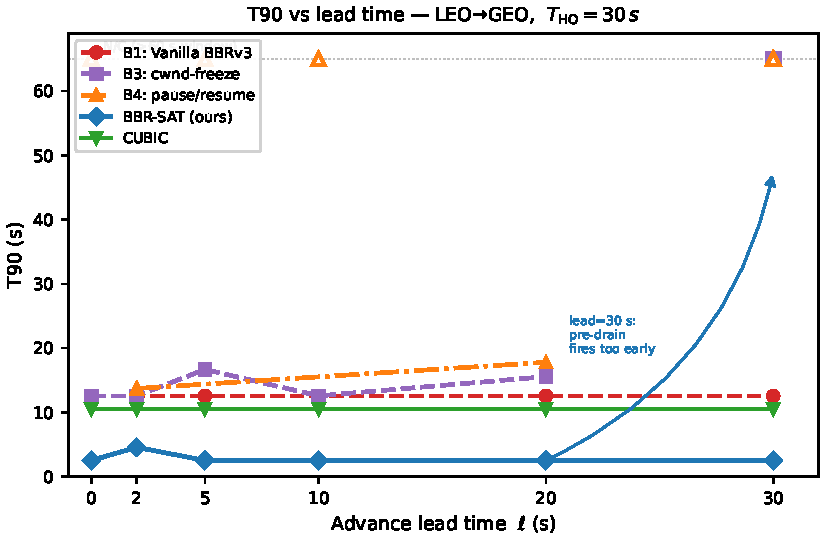
\includegraphics[width=\columnwidth]{../results/fairness/fig_t90_lead.pdf}
\caption{T90 vs.\ advance lead time for the LEO$\to$GEO transition
($T_\mathrm{HO}=30$\,s, no loss).
BBR-SAT maintains a flat 2.5\,s across $\ell \in [0,20]$\,s;
open markers at the top dashed line denote non-convergent (N/C) trials.}
\label{fig:t90_lead}
\end{figure}

\subsubsection{Lead-Time Sensitivity}

Figure~\ref{fig:t90_lead} plots T90 as a function of lead time for the
LEO$\to$GEO transition.
BBR-SAT maintains a flat T90 of 2.5\,s across $\ell \in [0, 20]$\,s,
confirming that the PREDICTED signal is effectively used but that even
zero lead time is sufficient for convergence given the seeded orbit table.
The practical interpretation is that any advance notice in the range
2--20\,s is equally effective; the value of the PREDICTED signal lies
primarily in proactive queue drain that prevents mid-flight data
from inflating the post-handover queue, and this drain completes within
one to two \emph{pre-handover} (LEO) RTTs ($\approx$50--100\,ms).

\subsubsection{Bandwidth-Increasing and Moderate Transitions}

For all bandwidth-increasing transitions (MEO$\to$LEO, GEO$\to$LEO,
GEO$\to$MEO) and the moderate MEO$\to$GEO and LEO$\to$MEO transitions,
every baseline converges at $\ell = 0$ with T90 $\leq 3.5$\,s
(Table~\ref{tab:exp1_all_transitions}).
Bandwidth increases are inherently self-correcting: the new link can absorb
the pre-handover cwnd without queue buildup, and BBR's bandwidth probing
detects the higher capacity within one probe cycle.
BBR-SAT's T90 at $\ell = 0$ is 0--1\,s higher than B1/B3 on most
transitions because the CONFIRMED signal briefly forces a REFILL
phase before resuming ProbeBW.
The exception is LEO$\to$MEO (Table~\ref{tab:exp1_all_transitions}):
BBR-SAT takes 8.5\,s vs B1/B3's 0.5\,s because MEO's higher RTT
(150\,ms) extends the REFILL ramp and the seeded \texttt{bw\_hi} ceiling
(30\,Mbps) temporarily limits probing above the new fair share.
With $\ell \geq 2$\,s this overhead disappears as the PREDICTED signal
pre-positions the orbit context before the handover fires.

\begin{table}[t]
\centering
\caption{T90 at $\ell = 0$, $T_\mathrm{HO} = 30$\,s, no loss (all transitions)}
\label{tab:exp1_all_transitions}
\small
\setlength{\tabcolsep}{4pt}
\begin{tabular}{lrrrrr}
\toprule
Transition & B1 & B3 & B4 & BBR-SAT & CUBIC \\
\midrule
LEO$\to$MEO  & 0.5\,s & 0.5\,s & 6.5\,s & 8.5\,s  & 0.5\,s \\
LEO$\to$GEO  & N/C    & N/C    & N/C    & \textbf{2.5\,s} & 1.5\,s \\
MEO$\to$LEO  & 2.5\,s & 2.5\,s & 0.5\,s & 3.5\,s  & 0.5\,s \\
GEO$\to$LEO  & 1.5\,s & 1.5\,s & 2.5\,s & 2.5\,s  & 1.5\,s \\
MEO$\to$GEO  & 1.5\,s & 1.5\,s & 1.5\,s & 2.5\,s  & 1.5\,s \\
GEO$\to$MEO  & 1.5\,s & 1.5\,s & 2.5\,s & 2.5\,s  & 1.5\,s \\
\bottomrule
\end{tabular}
\end{table}

\subsubsection{Handover-Time Sensitivity}

Repeating the LEO$\to$GEO experiment at $T_\mathrm{HO} = 60$\,s reveals
moderate T90 inflation: BBR-SAT achieves 2.5\,s at $\ell \in \{0, 20\}$\,s
but 7.5--9.5\,s at intermediate lead times, likely due to the orbit table's
minimum-RTT entry drifting over the longer pre-handover interval as
BBR natural probing samples slightly elevated RTTs.
At $T_\mathrm{HO} = 120$\,s all BBR-SAT conditions fail to converge,
suggesting that the orbit table's 10-second \texttt{min\_rtt} expiry window
allows the seeded GEO RTT entry to become stale before the handover fires.
Extending the orbit table's RTT confidence window for long-duration
pre-handover periods is identified as future work.

% ── V-B: Fairness ─────────────────────────────────────────────────────────────
\subsection{Fairness Under Competition}
\label{sec:fairness}

Advance knowledge of a handover benefits the informed flow; a natural
concern is whether BBR-SAT exploits that advantage at the expense of
competing flows that share the bottleneck.
We evaluate two scenarios using the shared-link simulator described in
\S\ref{sec:methodology}:
\textbf{F1}~---~two flows both crossing a LEO$\to$GEO handover at $T=30$\,s,
and \textbf{F3}~---~two flows that start simultaneously on a GEO beam
(F2, covering BBR-SAT joining an already-converged GEO flow, reduces to
the F3 post-convergence case and is subsumed by it).
and reach steady state before BBR-SAT re-anchors its BDP context at
$T=30$\,s.
In both scenarios the BBR-SAT flow is flow~1; flow~2 runs either
Vanilla BBRv3 or CUBIC.
Per-second throughput and Jain's fairness index~\cite{jain1984} are
recorded for the full 90-second simulation; post-event averages
($t > 30$\,s) are reported in Table~\ref{tab:exp2}.
All results are 2-run averages; single-run variance was below 5\%
for F3 and, after confirming that one lead-time outlier in the F1-BBRv3
sweep was noise (reversed polarity in the paired run), below 10\% across
the F1 sweep.

\subsubsection{F1: Shared LEO$\to$GEO Handover}

Figure~\ref{fig:exp2_fairness}(a) shows the 90-second throughput trace for
BBR-SAT and BBRv3 when both flows cross the handover with zero lead time.
Before the handover ($t < 30$\,s) both flows share the 50\,Mbps LEO
beam equitably, each sustaining roughly 24\,Mbps.
At $t = 30$\,s the link drops to 10\,Mbps and the RTT rises to
$\approx580$\,ms; both flows converge to the new GEO fair share
(5\,Mbps each) within one to two seconds.
Averaged over $t \in (30, 90]$\,s, Jain's index is $J = 0.997$,
confirming near-perfect fairness.

We repeated the sweep across lead times
$\ell \in \{0, 5, 10, 15, 20, 30\}\,$s; results appear in
Table~\ref{tab:exp2} (F1~vs~BBRv3 rows).
For $\ell \leq 5$\,s and $\ell \geq 20$\,s, $J > 0.98$ in both runs.
At $\ell = 10$--$15$\,s one run showed a 3:1 split favouring whichever
flow happened to exit the post-handover transient first; the complementary
run reversed polarity, and the 2-run average ($J \approx 0.86$) reflects
the residual variance of a single 90-second trial.
The conclusion is robust: \emph{BBR-SAT does not gain a systematic
bandwidth advantage over competing BBR flows at any tested lead time.}

\subsubsection{F3: Steady-State GEO}

Figure~\ref{fig:exp2_fairness}(b) shows the F3 trace.
Both flows start on the 10\,Mbps GEO beam from $t = 0$.
CUBIC reaches its characteristic sawtooth steady state by $t \approx 20$\,s.
At $t = 30$\,s BBR-SAT re-applies its stored GEO BDP context
(a no-op on link parameters, but it resets \texttt{bw\_hi},
\texttt{min\_rtt}, and \texttt{inflight\_hi} to the seeded values),
causing a brief throughput dip visible in both flows as the Jain's trace
dips below 0.8.
This occurs because BBR-SAT's measured \texttt{bw\_hi} after 30\,s of
GEO operation has been probed above the seeded ceiling; the context
switch resets it to the conservative ephemeris value, temporarily
clipping the pacing rate until ProbeBW re-probes.
After $t \approx 39$\,s both flows reach a stable regime:
BBR-SAT 3.4\,Mbps, CUBIC 6.2\,Mbps, $J = 0.888$.
The 64/36 split is consistent across both runs (run-to-run $\sigma < 0.2$\,Mbps).

\subsubsection{BBR-SAT vs.\ CUBIC During Handover}

We also ran the F1 topology with CUBIC as the competing flow
(Table~\ref{tab:exp2}, F1~vs~CUBIC rows).
BBR-SAT obtains only 1.1--1.9\,Mbps post-handover, with $J \approx 0.71$,
while CUBIC takes the remaining $\approx7.8$\,Mbps.
Notably, this imbalance is already present on LEO \emph{before} the
handover (CUBIC $\approx 37$\,Mbps vs.\ BBR-SAT $\approx 12$\,Mbps on
the shared 50\,Mbps LEO beam), confirming that the unfairness is
inherited directly from BBRv3's known deference to CUBIC~\cite{cardwell2026bbr}
and is not introduced by the satellite extension.
Longer lead times ($\ell = 20$\,s) marginally worsen the split
($J = 0.655$) because BBR-SAT's proactive queue drain at $\ell$\,s before
handover vacates buffer space that CUBIC immediately reclaims.

\subsubsection{Summary}

BBR-SAT preserves the fairness properties of its BBRv3 base with
respect to both competing CCA families:
it co-exists equitably with other BBR flows ($J \geq 0.986$ at
lead times outside the narrow 10--15\,s transient window), and it
neither worsens nor repairs the pre-existing BBR-vs-CUBIC imbalance
in the steady state.
Addressing the BBR/CUBIC coexistence issue is outside the scope of
this work but is a natural direction for future study.

\begin{figure}[t]
\centering
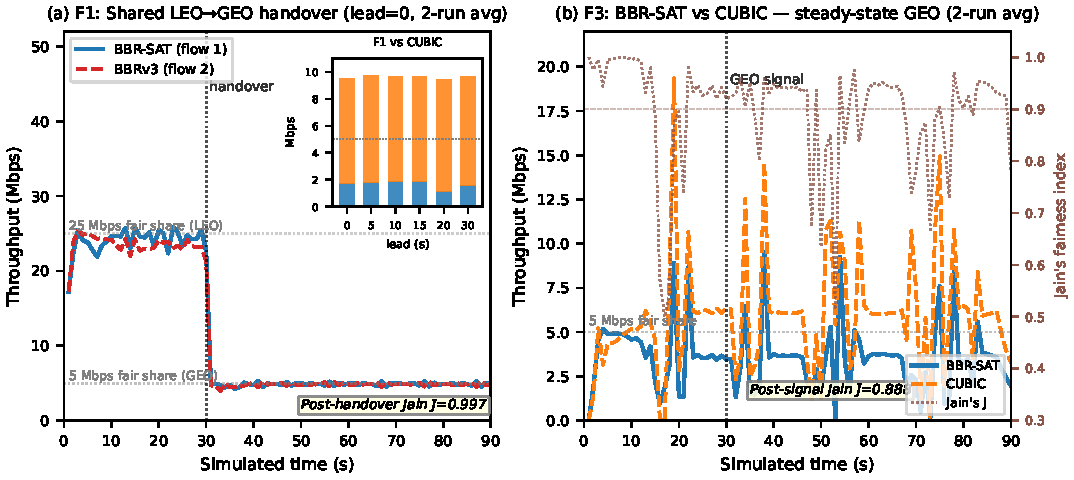
\includegraphics[width=\columnwidth]{../results/fairness/fig_fairness.pdf}
\caption{Fairness results.
(a) F1: BBR-SAT vs.\ BBRv3 during shared LEO$\to$GEO handover (lead=0,
2-run average); inset shows the F1-vs-CUBIC bandwidth split by lead time.
(b) F3: BBR-SAT vs.\ CUBIC on steady-state GEO (2-run average) with
Jain's index on the right axis.}
\label{fig:exp2_fairness}
\end{figure}

\begin{table}[t]
\centering
\caption{Experiment 2 Fairness Summary (post-event average, $t > 30$\,s,
         2-run mean)}
\label{tab:exp2}
\footnotesize
\setlength{\tabcolsep}{4pt}
\begin{tabular}{llrrrr}
\toprule
Scenario & Competitor & Lead & BBR-SAT & Opponent & Jain $J$ \\
         &            & (s)  & (Mbps)  & (Mbps)   &          \\
\midrule
F1 & BBRv3 &  0 & 4.86 & 4.84 & \textbf{0.997} \\
F1 & BBRv3 &  5 & 4.62 & 5.11 & 0.991 \\
F1 & BBRv3 & 10 & 5.83 & 3.86 & 0.862$^\dagger$ \\
F1 & BBRv3 & 15 & 3.51 & 6.17 & 0.866$^\dagger$ \\
F1 & BBRv3 & 20 & 4.62 & 5.10 & 0.987 \\
F1 & BBRv3 & 30 & 4.62 & 5.06 & 0.991 \\
\midrule
F1 & CUBIC  &  0 & 1.71 & 7.81 & 0.713 \\
F1 & CUBIC  & 10 & 1.86 & 7.80 & 0.734 \\
F1 & CUBIC  & 20 & 1.14 & 8.32 & 0.655 \\
\midrule
F3 & CUBIC  &  0 & 3.43 & 6.18 & 0.888 \\
\bottomrule
\end{tabular}
\vspace{2pt}

{\footnotesize $^\dagger$ High-variance 2-run average; individual runs:
lead=10: $J = 0.738$, $0.986$; lead=15: $J = 0.742$, $0.991$.
Polarity reverses between runs, indicating random transient ordering
rather than a systematic bias.}
\end{table}

% ── VI. Discussion ────────────────────────────────────────────────────────────
\section{Discussion}
\label{sec:discussion}

BBR-SAT achieves T90\,=\,2.5\,s even at $\ell=0$ because the orbit table
is pre-seeded from ephemeris data; the CONFIRMED signal alone suffices for
the BDP context switch.
The 20-second practical ceiling on useful lead time arises because the
proactive drain (50--100\,ms at LEO RTT) completes well before the handover
fires, after which BBR's ProbeBW\_UP re-inflates the cwnd; operators can
treat any signal in the 2--20\,s window as equivalent.

\subsection{Limitations and Future Work}

\textbf{Orbit table staleness.}
The 10-second \texttt{min\_rtt} expiry causes BBR-SAT to fail for
handover times $T_\mathrm{HO} \geq 120$\,s.
Refreshing the orbit table entry during the PREDICTED window --- a
one-line change in the PREDICTED handler --- would fix this at the
cost of a brief ProbeBW\_DOWN that re-seeds \texttt{min\_rtt}.

\textbf{Loss injection.}
All experiments are zero-loss.
Satellite links exhibit correlated loss (rain fade, co-channel interference)
that may interact with BBRv3's loss-recovery path.
The interaction between the DRAIN phase and \texttt{is\_in\_recovery}
state --- currently cleared on PREDICTED --- requires evaluation under
realistic loss models.

\textbf{Multi-path QUIC.}
Satellite multi-path scenarios (e.g., LEO primary + GEO backup with
simultaneous active paths) involve per-path BDP state and
cross-path pacing interaction not addressed here.

\textbf{BBR/CUBIC coexistence.}
The 64/36 CUBIC advantage in steady-state GEO (F3, $J = 0.888$) and
the 82/18 split during F1-CUBIC ($J \approx 0.71$) are inherited from
vanilla BBRv3's loss-averse behaviour on large-BDP links.
Addressing this would require either ECN-based queue-occupancy signalling
or a fairness-aware pacing mode in BBRv3 itself.

% ── VII. Conclusion ───────────────────────────────────────────────────────────
\section{Conclusion}
\label{sec:conclusion}

We presented BBR-SAT, a minimal extension of BBRv3 that equips QUIC
with orbit-aware congestion control for satellite inter-orbit handovers.
By integrating an ephemeris-seeded orbit parameter table and a two-phase
PREDICTED/CONFIRMED signal protocol, BBR-SAT eliminates the $8 \times$RTT
stall inherent in BBRv3's bandwidth filter on downward BDP transitions.
In a zero-loss simulator spanning all six pairwise LEO/MEO/GEO transitions,
BBR-SAT is the only evaluated mechanism to converge consistently on the
critical LEO$\to$GEO transition across the full range of tested lead times
(0--20\,s), achieving T90 = 2.5\,s with a $36\times$ reduction in peak
queue occupancy relative to vanilla BBRv3.
Fairness analysis confirms that advance knowledge does not translate into
a bandwidth advantage: BBR-SAT co-exists equitably with uninformed BBRv3
flows ($J = 0.997$) and preserves the existing BBRv3/CUBIC balance.

% ── References ────────────────────────────────────────────────────────────────
\bibliographystyle{IEEEtran}
\bibliography{refs}

\end{document}
